\section{Federated Trustworthiness Rank}
\label{sec:trust_ranking}

While FedTruthFinder learns the integrated event truth in a privacy-preserving manner, it brings a challenge in justifying participants' trustworthiness. For example, to incentivize the crowdsensing participants, it is a common strategy to pay the high-trustworthy participants (i.e., high-quality sensing results) with higher incentives. However, in FedTruthFinder, the sensing quality of each participant, i.e., the trustworthiness score $\tau_i$ is kept at each participant side and unknown to the server. Hence, how to assess participants' trustworthiness is required and challenging for FedTruthFinder.

In this section, we first illustrate a concrete case to describe that $\tau_i$ cannot be directly known to the server, otherwise the server may infer which event $u_i$ has sensed. As $\tau_i$ cannot be known to the server, we then design a secure ranking algorithm to let the server know every participant $u_i$'s ranking position of $\tau_i$ among all the participants without leaking $\tau_i$. Based on the ranked positions, the crowdsensing organizer can enable certain trustworthiness-aware incentive mechanisms, e.g., rewarding high-position participants with bonus, which can incentivize participants to compete with each other to get more high-quality sensed data \citep{Reddy2010ExaminingMF}.

\subsection{Privacy Leakage by Trustworthiness $\tau_i$}

Here, we illustrate an example to show the risk of revealing $\tau_i$ to the server for leaking participant $u_i$'s privacy.

Without the loss of generality, we assume that $u_1$'s $\tau_1 = 0.9$, and other $u_i$'s $\tau_i < 0.9\ (i\not=1)$. Suppose that one event $e_j$'s $\rho_j = 0.9$ after truth discovery, then we can easily infer that $u_1$ has sensed the event $e_j$ and the sensed result is $1$. This reveals the fact that $u_1$ has visited the location of $e_j$, leaking $u_1$'s location privacy.

Hence, participants cannot directly upload their $\tau_i$ to the server for incentive allocation. Next, we design a privacy-preserving method to enable trustworthiness-aware incentive allocation. 

\subsection{Secure Trustworthiness Leader-board}

While revealing $\tau_i$ may leak participants' private information, we propose a secure ranking algorithm to learn a  leader-board regarding participants' trustworthiness for facilitating trustworthiness-aware incentive allocation.

Secure ranking algorithms have been studied for decades; however, prior studies cannot be directly applied in our scenario for two reasons. First, the communication overheads are usually high. Second, prior studies mostly assume that all the network connections are stable for all the parties, but this is unrealistic for crowdsensing. 

Our secure ranking algorithm generally follows the design of \citet{tang2011secure}. However, the original design \citep{tang2011secure} cannot tolerate any participants to lose the network connections. We thus enhance it to ensure that the ranking algorithm can still work when certain participants lose connections.
The major steps of our federated trustworthiness leader-board generation mechanism are:

\textbf{Step 1}. First, we categorize all the participants into $(2t+1)$ groups, and thus each group includes $n/(2t+1)$ participants. We denote $gid(u)$ to refer to the group ID of participant $u$.

\textbf{Step 2}. For each user $u_i$, she shares $\tau_i$, $\tau_i^2$, ... , $\tau_i^{2t+1}$ with $(t+1, 2t+1)$-SSS to all the user groups. Specifically, a user $u_j$ will receive the share piece regarding $gid(u_j)$, denoted as $\tau_{i_1}(gid(u_j))$, $\tau_{i_2}(gid(u_j))$, ... $\tau_{i_{2t+1}}(gid(u_j))$ for $\tau_i$, $\tau_i^2$, ... , $\tau_i^{2t+1}$, respectively.

\textbf{Step 3}. For each user group $g_k$, it generates a random number $r_k (>0)$ and shares $r_k$ with $(t+1, 2t+1)$-SSS to all the user groups. That is, $u_j$ will receive $r_k$'s share regarding $gid(u_j)$, denoted as $r_k(gid(u_j))$.

\textbf{Step 4}. For each participant $u_j$, she calculates the following number with the $\tau_{i_k}(gid(u_j))$ received from $u_i$:
\begin{align}
h_{i}(gid(u_j)) &= \lambda(gid(u_j)) \sum_{k=1}^{2t+1} r_k(gid(u_j)) \tau_{i_k}(gid(u_j)) \\ &= \lambda(gid(u_j)) \gamma(gid(u_j))
\end{align}
where
\[
\left(\begin{array}{ccccc} 
	1 &    1 & 1^2 & ...  & 1^{2t} \\ 
	1 &    2 & 2^2 & ... & 2^{2t}\\
	... & ... & ... & ...& ...\\
	1 & 2t+1 & (2t+1)^2 & ... & (2t+1)^{2t}\\
\end{array}\right)^{-1} 
\]
\[
=\left(\begin{array}{ccccc} 
	\lambda(1) &   \lambda(2) & \lambda(3) & ...  & \lambda(2t+1) \\ 
	... & ... & ... & ...& ...\\
	... & ... & ... & ...& ...\\
	... & ... & ... & ...& ...
\end{array}\right) 
\]


\textbf{Step 5}. For each user group, we randomly select one participant $u_j$ to share $\{h_{i}(gid(u_j))| i \in [1,n]\}$ with $(t+1, n)$-SSS to all the $n$ participants. Each user $u_k$'s received shares from all the groups are denoted as $\{h_i(g, k)| i \in [1,n], g \in [1, 2t+1]\}$.

\textbf{Step 6}. For each participant $u_k$, she computes:
\begin{equation}
h'_i(k) = \sum_{g=1}^{2t+1} h_i(g, k), \quad \forall i \in [1,n]
\end{equation}
Each $u_k$ sends $\{h'_i(k)| i\in[1,n]\}$ to the server.

\textbf{Step 7}. After receiving at least $t+1$ participants' $\{h'_i(k)| i\in[1,n]\}$, the server can recover:
\begin{equation}
	h_i = \sum_{k=1}^{2t+1} r_k \tau_i^k, \quad \forall i \in [1,n]
\end{equation}

\textbf{Step 8}. The server ranks $u_i$ according to $h_i$ and the ranked list is the leader-board regarding trustworthiness $\tau_i$.

Note that same as $\rho$-computation, we do not need to establish the peer-to-peer communication channels between every two participant clients and can use the crowdsensing server for coordination. To avoid redundancy, readers can refer to Sec.~\ref{subsub:server_coordination} for details.

\textbf{Remark on our novelty}. The key improvement of our secure ranking algorithm compared to \citet{tang2011secure} is the enhanced robustness against participants' connection loss. In \citet{tang2011secure}, every participant holds a $r_i$ and we will randomly select $2t+1$ participants to share their $r_i$ (Step 3) and $h_i$ (Step 5). This process is easy to break if a selected online user (Step 3) loses the connection in Step 5. Our proposed algorithm first constructs user groups so that we only need at least one participant online in each group for both Step 3 and 5, reducing the failure possibility incurred by connection loss. It is worth noting that this algorithm can not only rank crowdsensing participants' trustworthiness, but also be applied to many other applications when privacy-preserving data ranking is needed under unstable network connections.

\textbf{Remark on the ranked measurements}. In the previous algorithm description, we suppose that $\tau_i$ needs to be ranked. In practice, crowdsensing organizers can use the same secure ranking mechanism to rank other key measurements of participants (e.g., the number of sensed events) to design better incentive mechanisms or participant recruitment strategies.

\subsection{Theoretical Analysis}
\label{sub:theoretical_analysis_2}

All the proofs are illustrated in Appendix.

\subsubsection{Correctness} We first prove the correctness of our algorithm.

\vspace{+.5em}
\textbf{Lemma 5.1}. $\sum_{k=1}^{2t+1} r_k(x)\tau_{i_k}(x)$ can be represented as:
$$h_{i}+a_{i1}x+a_{i2}x^2+...+a_{i2t}x^{2t}$$
where $h_i=\sum_{k=1}^{2t+1} r_k\tau_i^k$. \citep{tang2011secure}
 
\vspace{+.5em}
\textbf{Theorem 5.1}. With $t+1$ participants' $h'_i(k)$, we can recover $h_i$.

\begin{figure*}[t!]%[tbhp]
	\centering
		\begin{subfigure}[t]{.325\linewidth}
			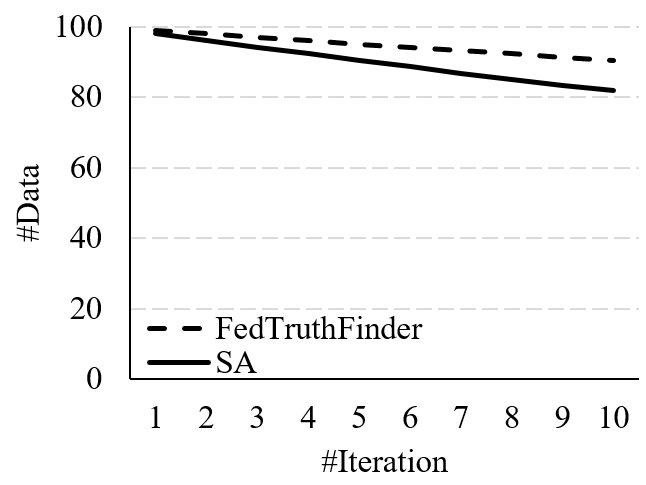
\includegraphics[width=1\linewidth]{./fig/data_num_cl0.01.PNG}
			\caption{$p_l=0.01$}
			\label{fig:cl0.01}
		\end{subfigure}
		\begin{subfigure}[t]{.325\linewidth}
			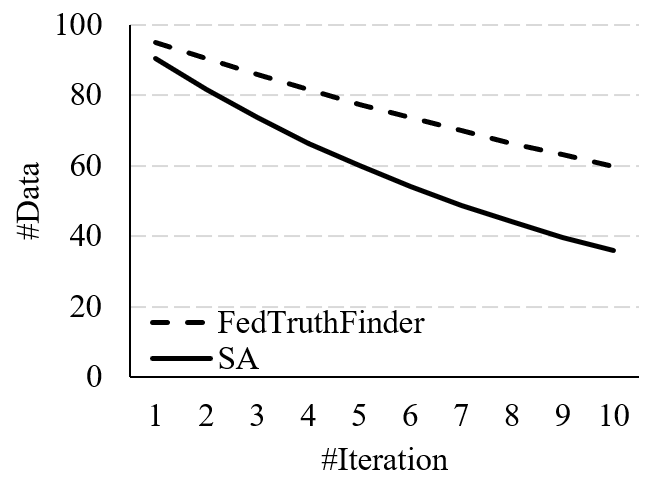
\includegraphics[width=1\linewidth]{./fig/data_num_cl0.05.PNG}
			\caption{$p_l=0.05$}
			\label{fig:chicago}
		\end{subfigure}
		\begin{subfigure}[t]{.325\linewidth}
			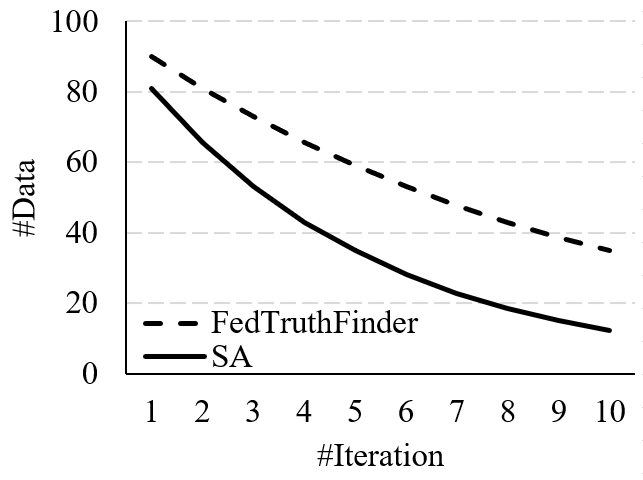
\includegraphics[width=1\linewidth]{./fig/data_num_cl0.1.PNG}
			\caption{$p_l=0.1$}
			\label{fig:dc}
		\end{subfigure}
		\caption{Number of data for each event's truth discovery by iterations.}
		\label{fig:num_sensed_data}
\end{figure*}

\begin{figure*}
	\centering
		\begin{subfigure}[t]{.3\linewidth}
			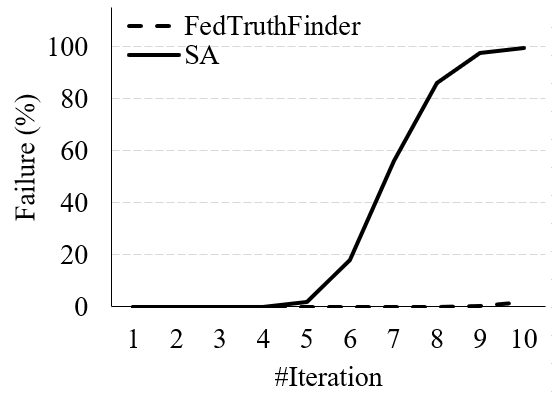
\includegraphics[width=1\linewidth]{./fig/failure_cl0.05.PNG}
			\caption{$p_l=0.05$}
		\end{subfigure}
		\begin{subfigure}[t]{.3\linewidth}
			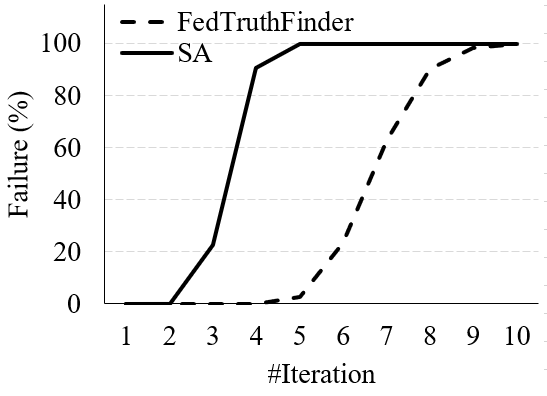
\includegraphics[width=1\linewidth]{./fig/failure_cl0.1.PNG}
			\caption{$p_l=0.1$}
		\end{subfigure}
		\caption{Failure probability of truth discovery.}
		\label{fig:failure}
\end{figure*}

\vspace{+.5em}
\textbf{Theorem 5.2}. Ranking $h_i$ is equivalent to ranking $\tau_i$.


\subsubsection{Robustness to Connection Loss} We analyze how our secure ranking algorithm can tolerate connection losses. We assume that before Step 2, there is no user connection loss.\footnote{If $u_i$ loses the connection in Step 2 and cannot share $\tau_i^k$ with SSS, then there is no way to rank $u_i$'s position because the server has no $u_i$'s information.}

\vspace{+.5em}
\textbf{Theorem 5.3}. To finish Step 3-5, there needs at least one user online for each group. Suppose that every user has $p_l$ probability to lose connection and there are $n$ users, the success probability $\ge (1-p_l^{\lfloor n/(2t+1) \rfloor})^{2t+1}$.


\vspace{+.5em}
\textbf{Theorem 5.4}. To finish Step 6-8, $\ge t+1$ users need to be online.



\subsubsection{Security} Here, we analyze the security of our mechanism.

\vspace{+.5em}
\textbf{Theorem 5.5} If there are no more than $t$ collusive participants, then these participants cannot recover all the other users' $\tau_i$.






\subsubsection{Complexity} We analyze the algorithm from communication and computation complexity perspectives for participant clients.

\textbf{Communication Complexity - $O(tn)$}. In Step 2, the communication overhead of one participant to send $\tau_i,\tau_i^2,...,\tau_i^{2t+1}$ is $O(t^2)$, while each user received data is $O(tn)$. In Step 3, the complexity is $O(t)$. In Step 5, for sending data, the complexity is $O(n)$; for receiving data, the complexity is $O(tn)$. In Step 7, the complexity is $O(n)$. Combing them together, the communication complexity of the whole process is $O(tn)$ as $t<n$.


\textbf{Computation Complexity - $O(tn)$}. The main computation processes of each client include (1) calculating secret shares for $\tau_i,\tau_i^2,...,\tau_i^{2t+1}$ with $(t+1, 2t+1)$-SSS in Step 2, which is $O(t^2)$, (2) calculating secret shares of $r_k$ in Step 3, which is $O(t)$, (3) computing  $h_i$ in Step 4, which is $O(tn)$, and (4) calculating $h_i'$ in Step 6, which is $O(tn)$. Hence, the final computation complexity is $O(tn)$.
